\documentclass[tikz,border=6pt]{standalone}
\usepackage{tikz}
\usepackage{helvet}
\renewcommand{\familydefault}{\sfdefault}
\usetikzlibrary{positioning,arrows.meta,fit,backgrounds,calc}

\begin{document}
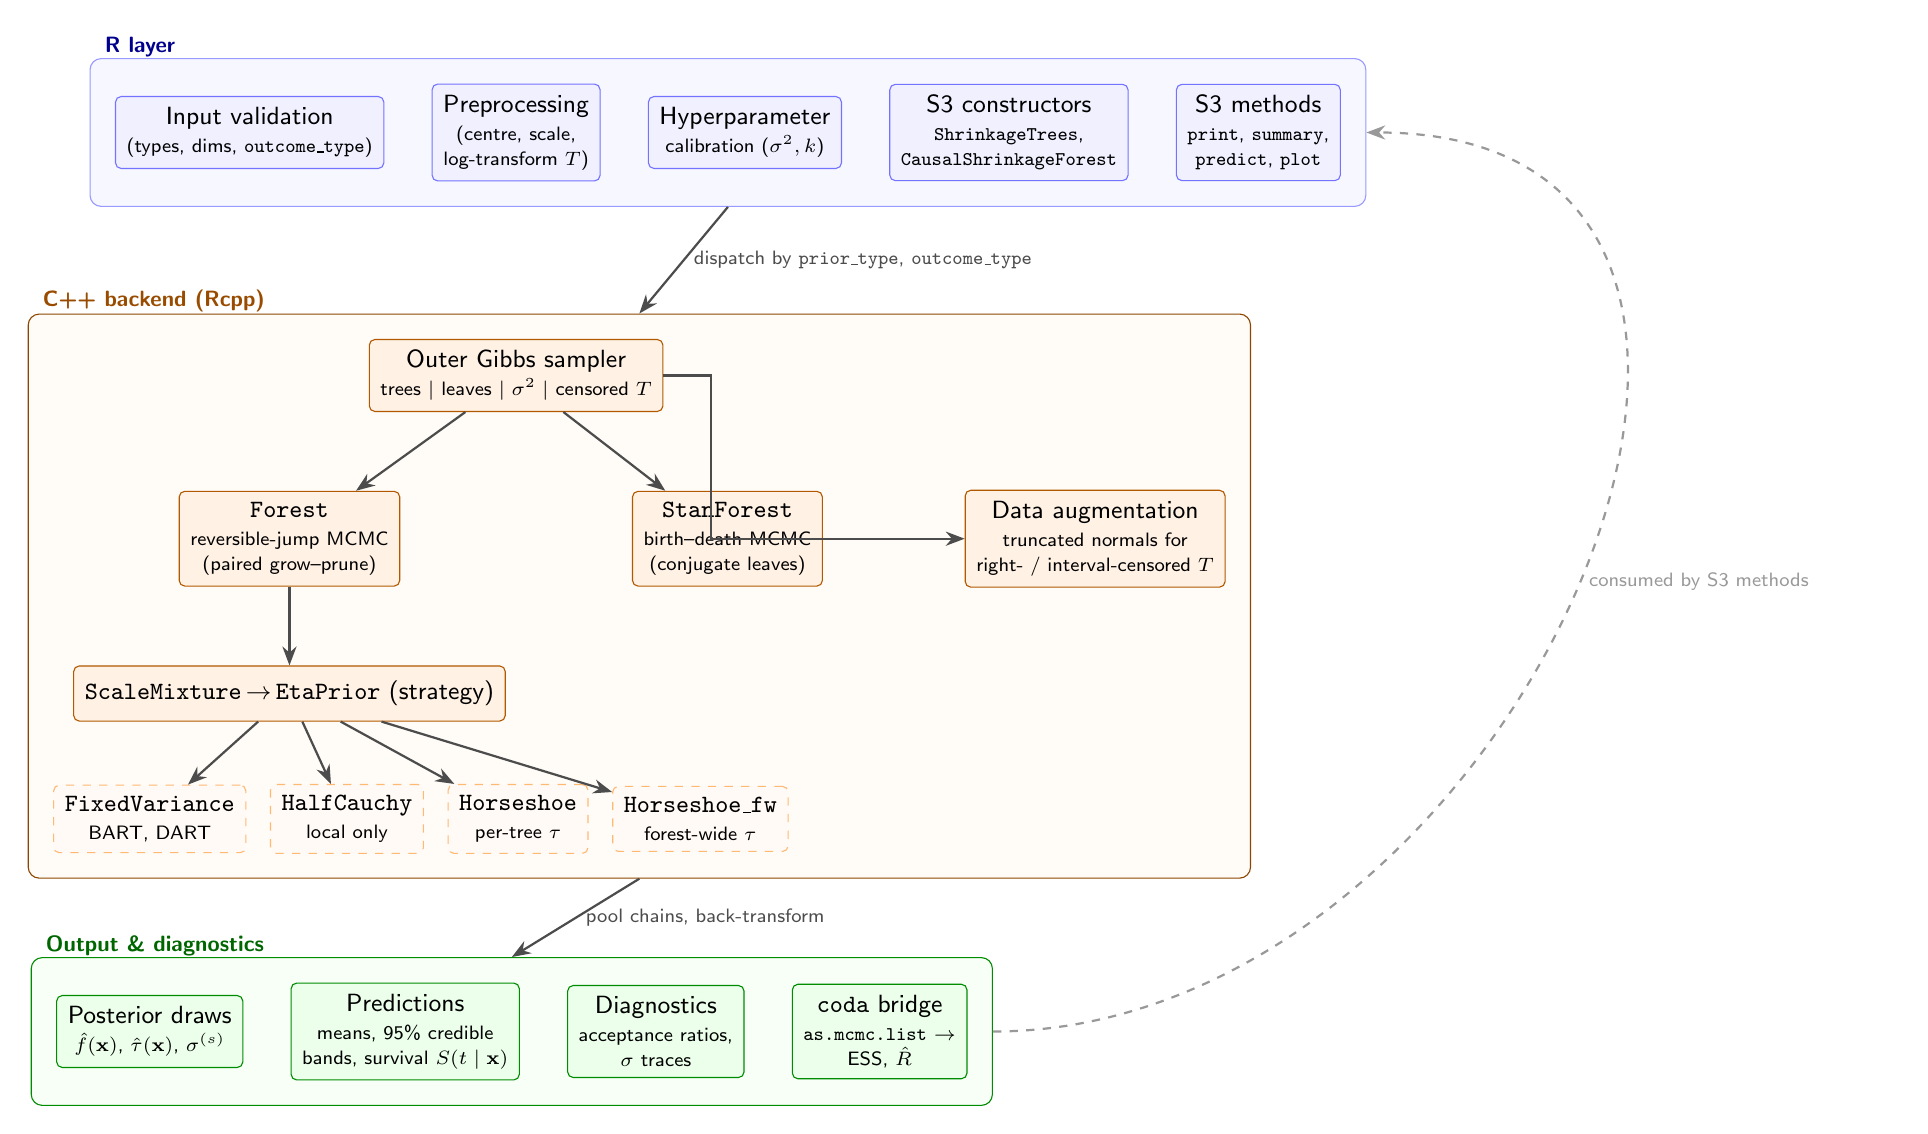
\begin{tikzpicture}[
  font=\small,
  >={Stealth[length=2.4mm,width=1.8mm]},
  layerlabel/.style={font=\bfseries\footnotesize, anchor=west},
  box/.style={
    draw=black!70, rounded corners=2pt, align=center,
    inner sep=4pt, minimum height=7mm, fill=white
  },
  rbox/.style={box, fill=blue!6,  draw=blue!55},
  cbox/.style={box, fill=orange!10, draw=orange!70!black},
  pbox/.style={box, fill=orange!4,  draw=orange!55, dashed},
  obox/.style={box, fill=green!8,  draw=green!55!black},
  arrow/.style={->, thick, black!70},
  faint/.style={->, thick, black!40, dashed}
]

% ---------- R LAYER ----------
\node[rbox] (valid)   {Input validation\\[-1pt]\scriptsize (types, dims, \texttt{outcome\_type})};
\node[rbox, right=6mm of valid] (prep)  {Preprocessing\\[-1pt]\scriptsize (centre, scale,\\[-2pt]\scriptsize log-transform $T$)};
\node[rbox, right=6mm of prep]  (hyper) {Hyperparameter\\[-1pt]\scriptsize calibration ($\sigma^2,k$)};
\node[rbox, right=6mm of hyper] (s3c)   {S3 constructors\\[-1pt]\scriptsize \texttt{ShrinkageTrees},\\[-2pt]\scriptsize \texttt{CausalShrinkageForest}};
\node[rbox, right=6mm of s3c]   (s3m)   {S3 methods\\[-1pt]\scriptsize \texttt{print}, \texttt{summary},\\[-2pt]\scriptsize \texttt{predict}, \texttt{plot}};

\begin{scope}[on background layer]
  \node[fit=(valid)(prep)(hyper)(s3c)(s3m),
        draw=blue!40, rounded corners=4pt, inner sep=9pt,
        fill=blue!3] (Rlayer) {};
\end{scope}
\node[layerlabel, blue!55!black] at (Rlayer.north west) [above right=-3pt and 2pt] {R layer};

% ---------- C++ LAYER ----------
% Sampler dispatch
\node[cbox, below=20mm of prep] (gibbs) {Outer Gibbs sampler\\[-1pt]\scriptsize trees $\mid$ leaves $\mid\sigma^2\mid$ censored $T$};

% Two forest implementations
\node[cbox, below left=10mm and -4mm of gibbs]  (rjforest) {\texttt{Forest}\\[-1pt]\scriptsize reversible-jump MCMC\\[-2pt]\scriptsize (paired grow--prune)};
\node[cbox, below right=10mm and -4mm of gibbs] (stan)     {\texttt{StanForest}\\[-1pt]\scriptsize birth--death MCMC\\[-2pt]\scriptsize (conjugate leaves)};

% ScaleMixture / EtaPrior
\node[cbox, below=10mm of rjforest] (sm) {\texttt{ScaleMixture}\,$\to$\,\texttt{EtaPrior} (strategy)};
\node[pbox, below left=8mm and -22mm of sm] (fv) {\texttt{FixedVariance}\\[-1pt]\scriptsize BART, DART};
\node[pbox, right=3mm of fv]              (hc) {\texttt{HalfCauchy}\\[-1pt]\scriptsize local only};
\node[pbox, right=3mm of hc]              (hs) {\texttt{Horseshoe}\\[-1pt]\scriptsize per-tree $\tau$};
\node[pbox, right=3mm of hs]              (hsfw) {\texttt{Horseshoe\_fw}\\[-1pt]\scriptsize forest-wide $\tau$};

% Censoring augmentation
\node[cbox, right=18mm of stan] (aug) {Data augmentation\\[-1pt]\scriptsize truncated normals for\\[-2pt]\scriptsize right- / interval-censored $T$};

\begin{scope}[on background layer]
  \node[fit=(gibbs)(rjforest)(stan)(sm)(fv)(hsfw)(aug),
        draw=orange!55!black, rounded corners=4pt, inner sep=9pt,
        fill=orange!3] (Clayer) {};
\end{scope}
\node[layerlabel, orange!60!black] at (Clayer.north west) [above right=-3pt and 2pt] {C++ backend (Rcpp)};

% Internal C++ arrows
\draw[arrow] (gibbs)    -- (rjforest);
\draw[arrow] (gibbs)    -- (stan);
\draw[arrow] (gibbs.east) -- ++(6mm,0) |- (aug.west);
\draw[arrow] (rjforest) -- (sm);
\draw[arrow] (sm) -- (fv);
\draw[arrow] (sm) -- (hc);
\draw[arrow] (sm) -- (hs);
\draw[arrow] (sm) -- (hsfw);

% ---------- OUTPUT LAYER ----------
\node[obox, below=18mm of fv]                (post)  {Posterior draws\\[-1pt]\scriptsize $\hat f(\mathbf{x})$, $\hat\tau(\mathbf{x})$, $\sigma^{(s)}$};
\node[obox, right=6mm of post]               (preds) {Predictions\\[-1pt]\scriptsize means, 95\% credible\\[-2pt]\scriptsize bands, survival $S(t\mid\mathbf{x})$};
\node[obox, right=6mm of preds]              (diag)  {Diagnostics\\[-1pt]\scriptsize acceptance ratios,\\[-2pt]\scriptsize $\sigma$ traces};
\node[obox, right=6mm of diag]               (coda)  {\texttt{coda} bridge\\[-1pt]\scriptsize \texttt{as.mcmc.list} $\to$\\[-2pt]\scriptsize ESS, $\hat R$};

\begin{scope}[on background layer]
  \node[fit=(post)(preds)(diag)(coda),
        draw=green!55!black, rounded corners=4pt, inner sep=9pt,
        fill=green!3] (Olayer) {};
\end{scope}
\node[layerlabel, green!40!black] at (Olayer.north west) [above right=-3pt and 2pt] {Output \& diagnostics};

% ---------- Cross-layer arrows ----------
\draw[arrow] (Rlayer.south) -- ($(Clayer.north)+(0,0)$)
  node[midway, right, font=\scriptsize] {dispatch by \texttt{prior\_type}, \texttt{outcome\_type}};
\draw[arrow] (Clayer.south) -- ($(Olayer.north)+(0,0)$)
  node[midway, right, font=\scriptsize] {pool chains, back-transform};
\draw[faint] (Olayer.east) to[out=0,in=0, looseness=1.4]
  node[midway, right, font=\scriptsize] {consumed by S3 methods}
  (Rlayer.east);

\end{tikzpicture}
\end{document}
